\section{Relaxation measurements - Franzen method}
\subsection{Set-up and procedure}
\begin{figure}
\centering
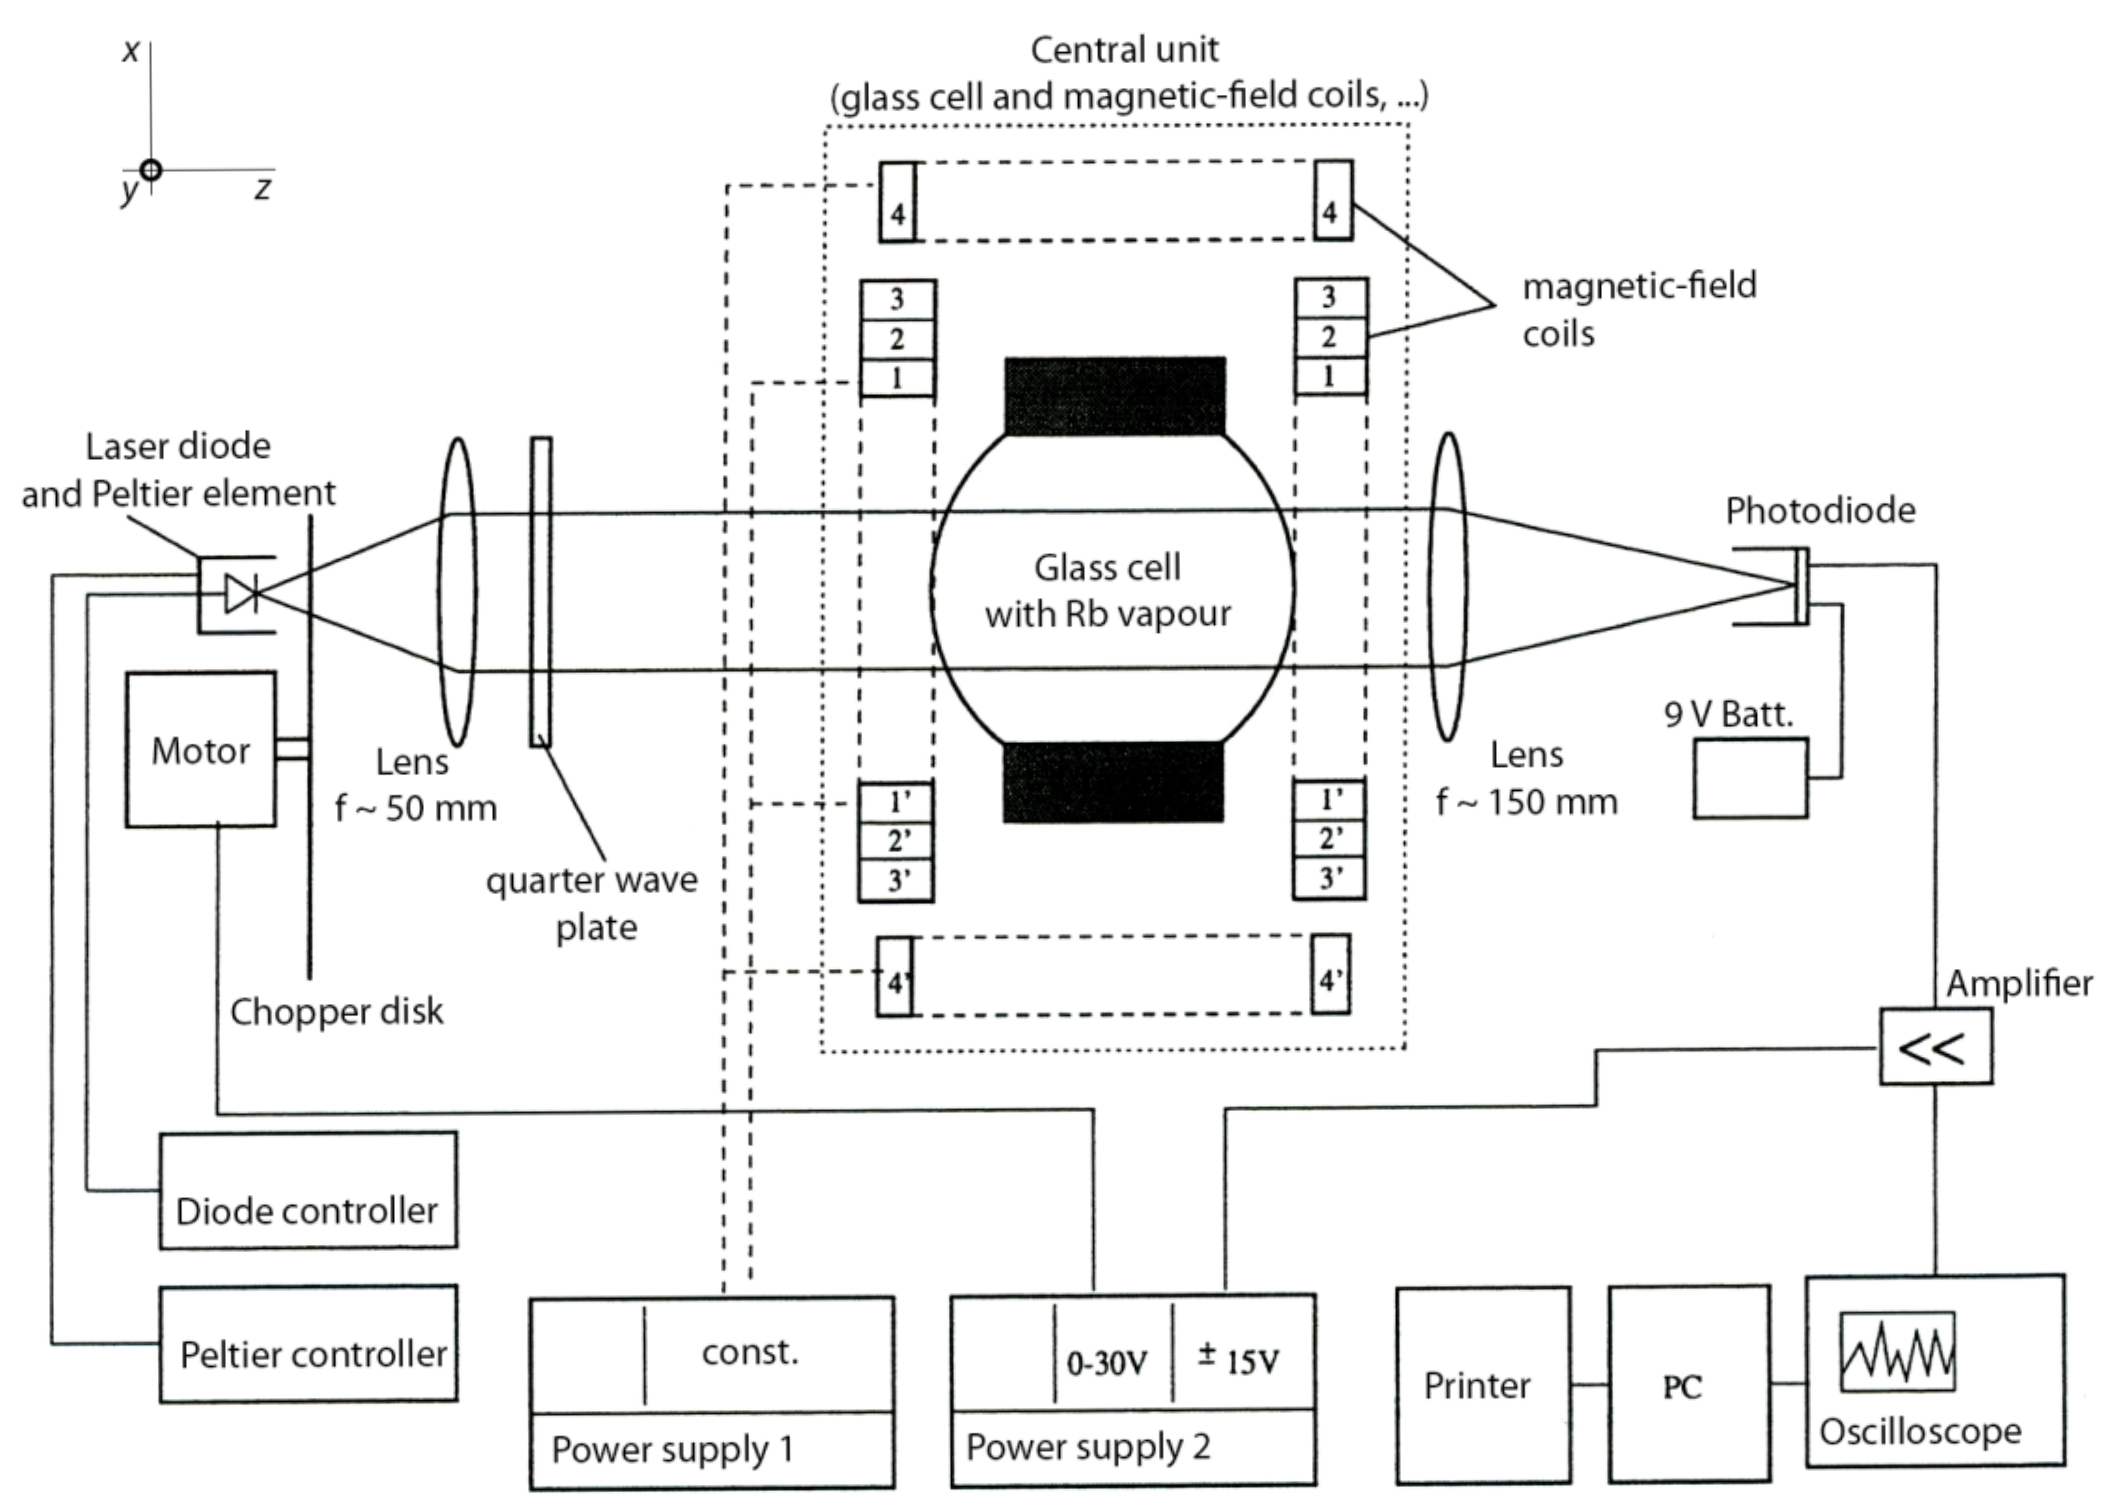
\includegraphics[width=1.0\linewidth]{graphics/franzensetup}
\caption[Set-up relaxation measurements - Franzen]{Set-up for the relaxation measurements with the Franzen method. The laser beam is periodicallz blocked with the chopper.\cite{anleitung}}
\label{fig:franzensetup}
\end{figure}
The Franzen method of determining the relaxation time relies on completely blocking and transmitting the laser. During the time when the laser is blocked ("darkness"), the system relaxes and, once the laser is transmitted again, causes exponentially dissipating absorption. The value from which the absorption reduces exponentially depends on the time for which the system was in darkness. The periodic blocking of the laser is facilitated by the chopper disk, which is placed as close to the laser as possible to make the cutting process faster. The laser current is set to maximize absorption signals.

\subsection{Data Analysis}
Measurements were taken at $T=\unit{34.3}{\degree}$ and $I_L=\unit{60.4}{mA}$. The vertical component of the earths' magnetic field remains compensated. For very low chopper voltages, the chopper signal was unstable and it was concluded that the motor does not operate steadily for such voltages. Measurements were then taken for motor voltages between $\unit{4}{V}$ and \unit{value}{unit}.
The results of one such measurement can be seen in figure 
For the fits, a Fermi function with a constant offset was used to approximate the intensity modulation by the chopper
\begin{equation}
I_{Ch}(t)=\frac{A}{1+e^{\frac{\mu-x}{\sigma}}}+U
\end{equation}
The relaxation, described by an exponential function, was made to start as soon as the Fermi function reaches 1\% intensity, which is true for $x>\mu-\sigma\log(99)$:
\begin{equation}
	I_R(t)=\begin{cases}
	0 &t\leq\mu-\sigma\log(99)\\
	B\cdot(1-e^{-\lambda(t-\mu)})&t\ge\mu-\sigma\log(99)
	\end{cases}
\end{equation}
\begin{figure}[htb]
	\centering
	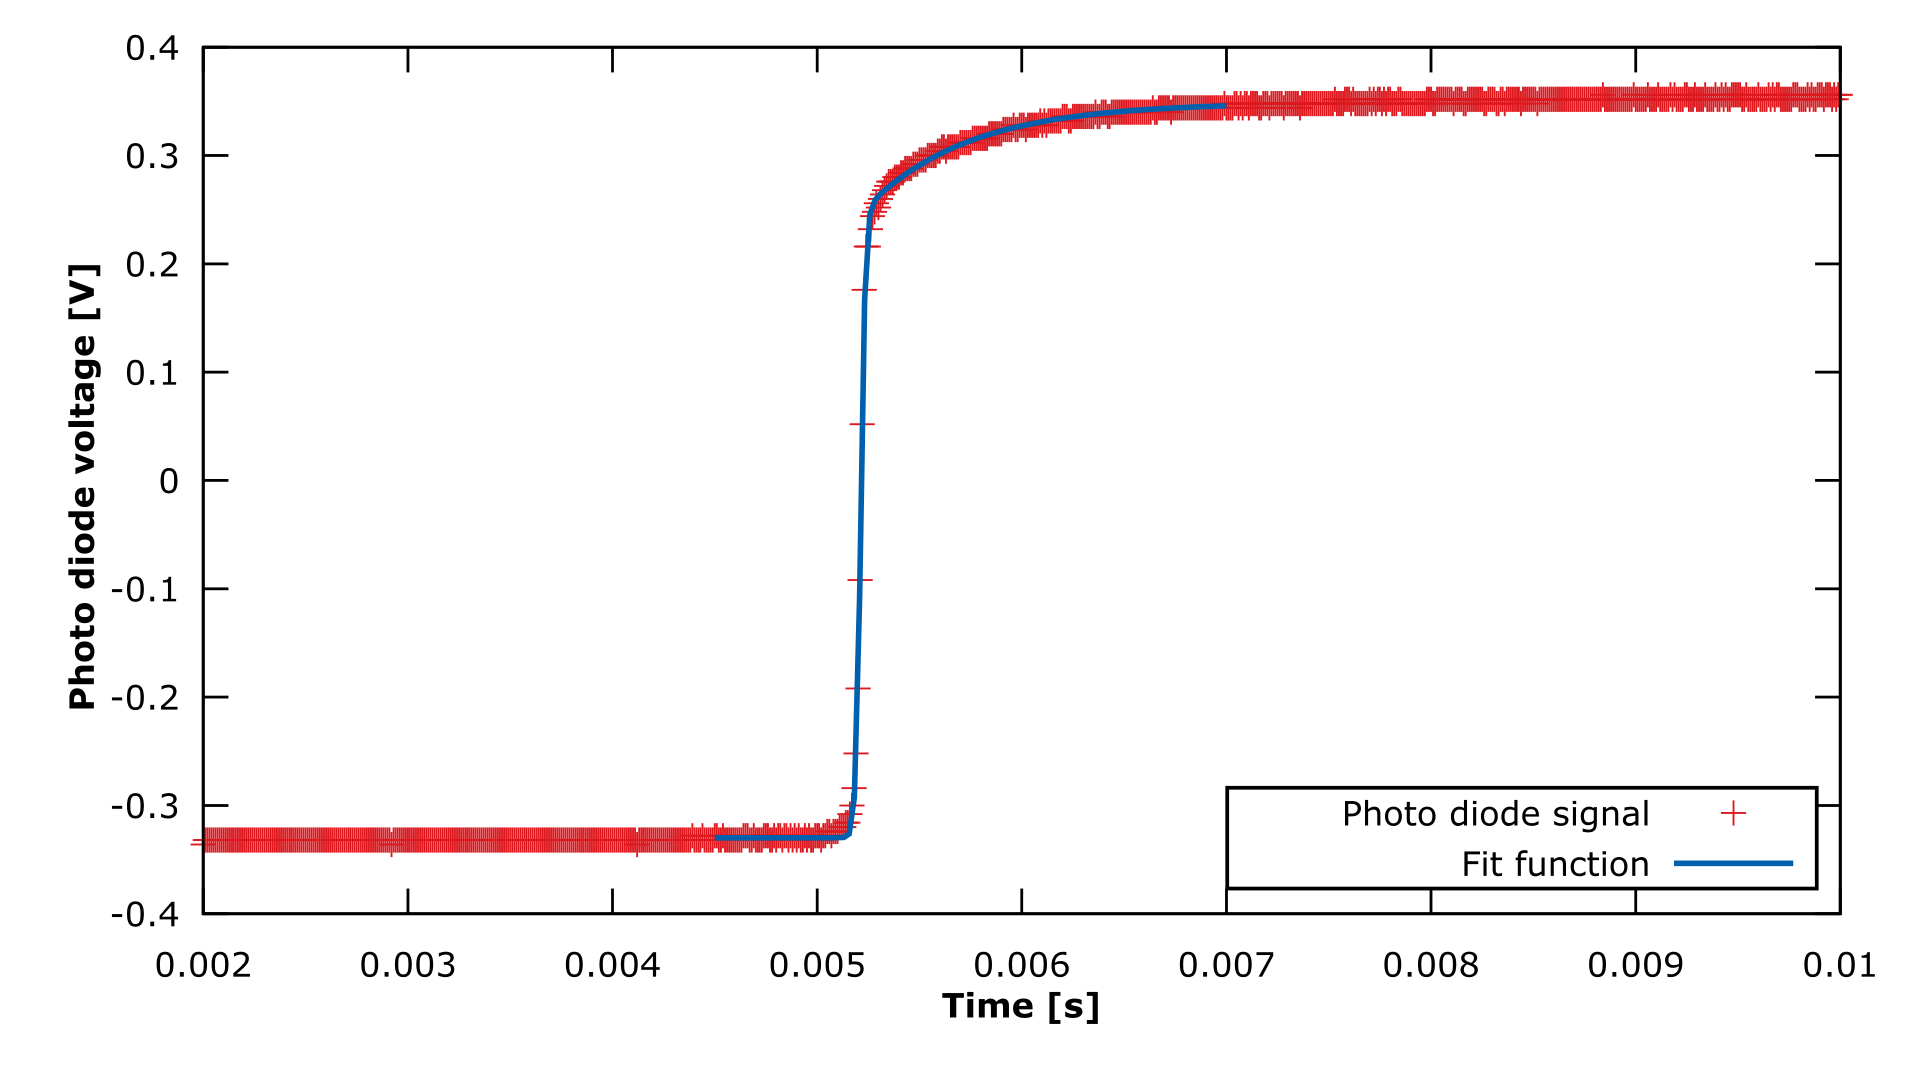
\includegraphics[width=1.0\linewidth]{graphics/franzenexample}
	\caption[Example of Franzen relaxation]{The relaxation measurement for a chopper voltage of \unit{4}{V} and the according fit.}
	\label{fig:franzenexample}
\end{figure}


These fits were very sensible to the starting parameters. The parameter $B$ is the absorption at $t=\mu-\sigma\log(99)$ and thus the sought after parameter. The dark times $t_d$ were taken from the data by hand and an uncertainty estimated each time. The parameter B for the different dark times can be seen in figure \ref{fig:Bparfit}. A fit of the form
\begin{equation}
B(t_d)=a+b\cdot(1-e^{-\frac{t_d}{T_R}})
\end{equation} 
where $a$ is an offset and $b$ is the amount of relaxation for large $t_d$. The data however is very linear and the fit thus converges only for very large $T_R$. The result for the relaxation time was
\begin{equation}
T_R=\unit{(50\pm24\cdot10^5)}{s}
\end{equation}

\begin{figure}
	\centering
	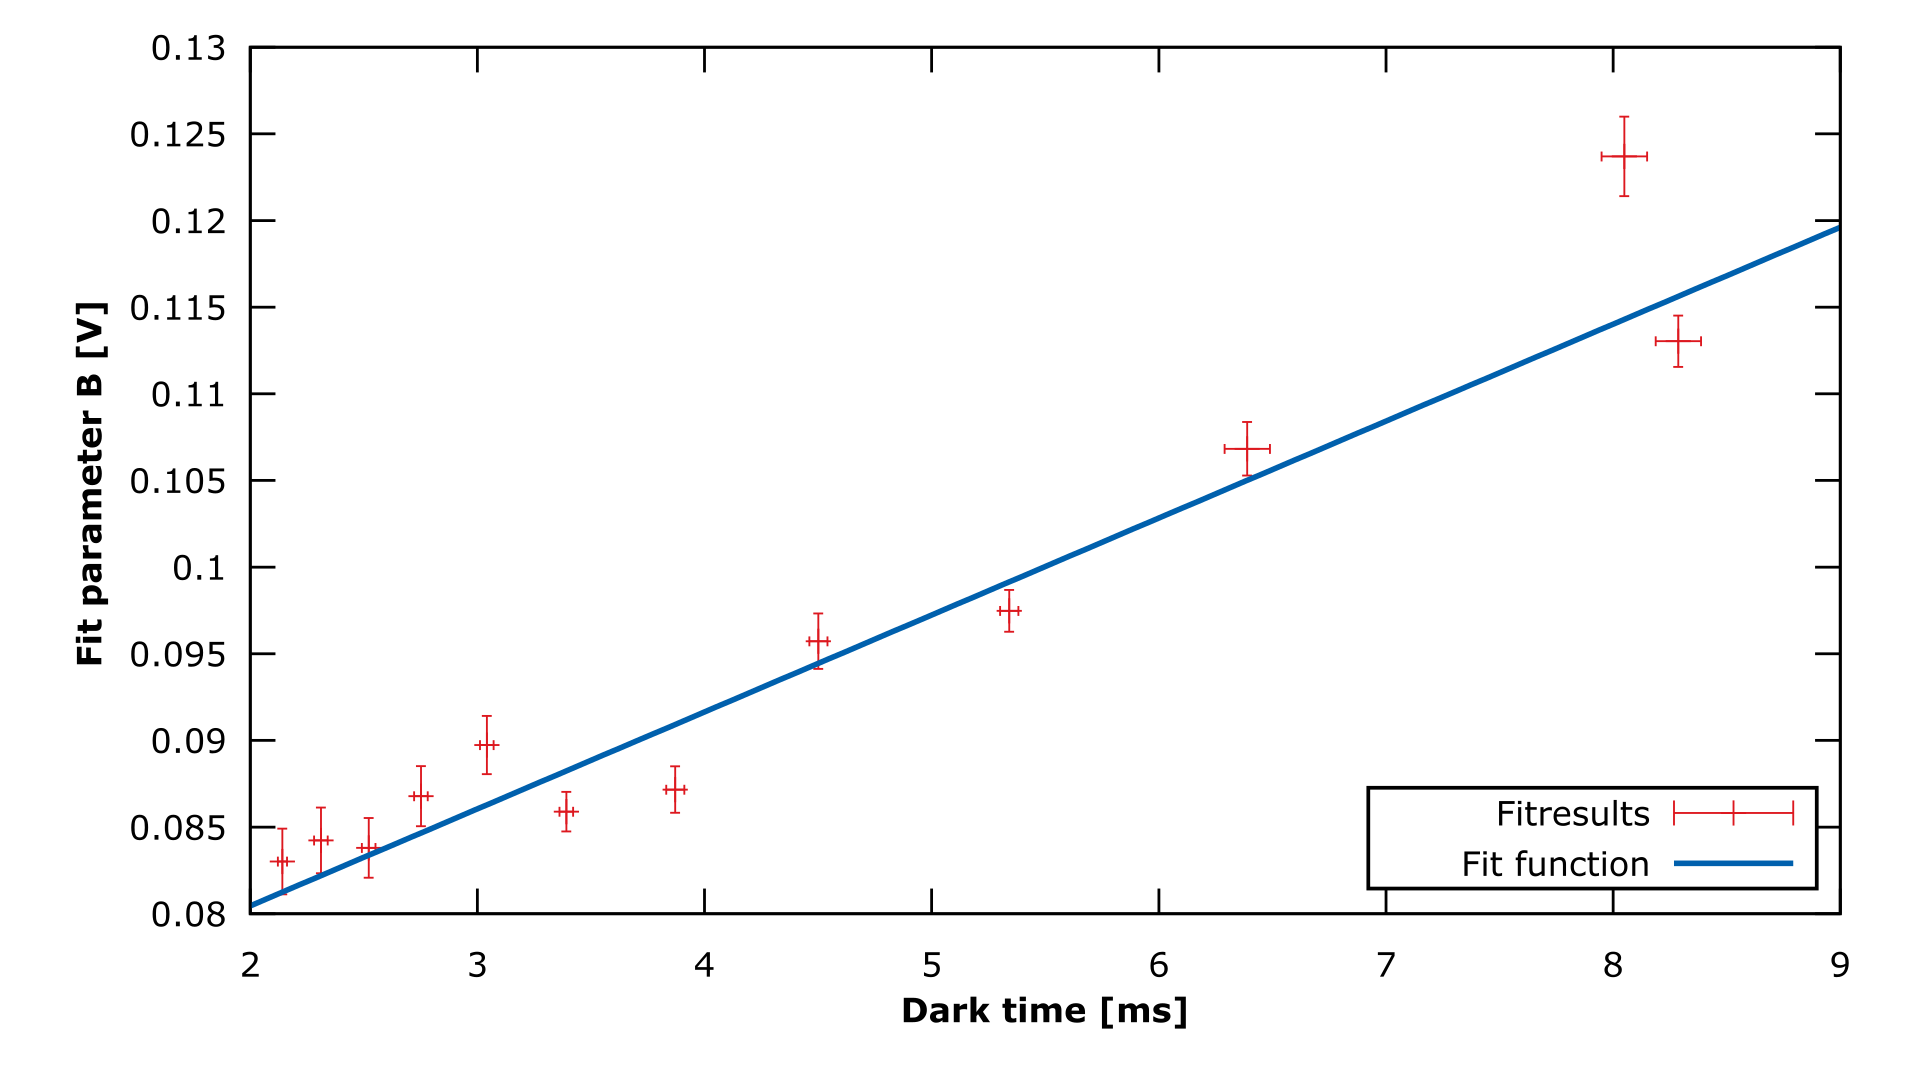
\includegraphics[width=1.0\linewidth]{graphics/Bparfit}
	\caption[Relaxation time fit Franzen]{The calculated fit parameters $B$ for the respective dark times.}
	\label{fig:Bparfit}
\end{figure}

Not only is the error astronomically large, the value is also several orders of magnitude away from the expected value of $T_R^{lit}=\unit{6.5}{ms}$. Longer dark times would likely have been needed for better measurements, but as mentioned before, the motor was not completely reliable for voltages below \unit{3}{V}. Figure \ref{fig:chopper1} shows the signal for \unit{1.5}{V}. The time that the edge of one opening in the chopper takes to fully pass by the laser is roughly \unit{0.5}{ms} and thus a significant time compared to the expected relaxation time of \unit{6.5}{ms}. Furthermore, the dark and light times seemed rather inconsistent, suggesting that the motor maybe does not operate at a constant speed. 



\begin{figure}
\centering
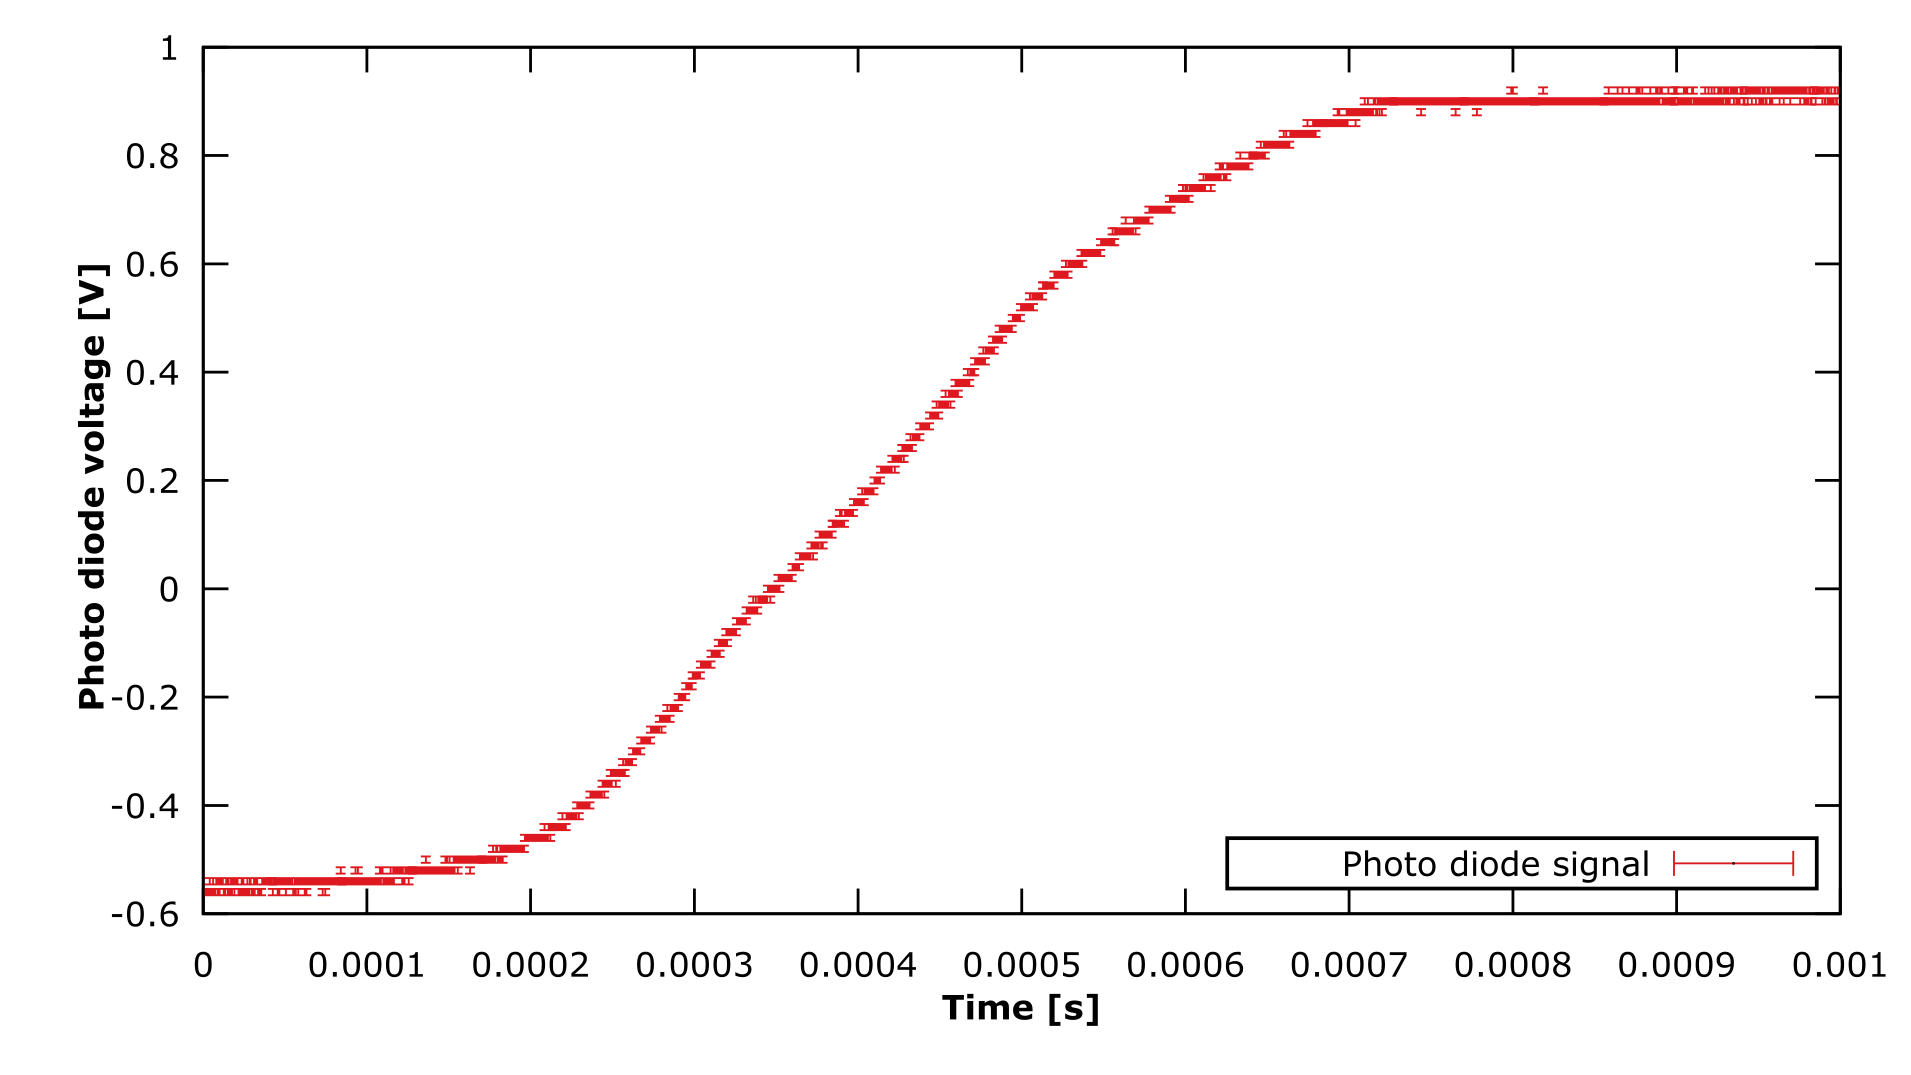
\includegraphics[width=1.0\linewidth]{graphics/chopper1,5V}
\caption[Chopper signal 1.5V]{The chopper signal for a supply voltage of \unit{1.5}{V}. The chopper takes roughly \unit{0.5}{ms} to fully pass by the laser. This is a significant time for the measurement period.}
\label{fig:chopper1}
\end{figure}




